\documentclass[12pt,a4paper]{article}
 \usepackage[utf8]{inputenc}
\usepackage{tikz}
\usetikzlibrary{shapes.geometric, arrows}
\tikzstyle{startstop} = [rectangle, rounded corners, minimum width=3cm, minimum height=1cm,text centered, draw=black, fill=red!30]
\tikzstyle{io} = [trapezium, trapezium left angle=80, trapezium right angle=100, minimum width=3cm, minimum height=1cm, text centered,  text width=2cm, draw=black, fill=blue!30]
\tikzstyle{process} = [rectangle, minimum width= 2.5cm, minimum height=1cm, text centered, text width=3cm, draw=black, fill=orange!30]
\tikzstyle{decision} = [diamond, minimum width=3cm, minimum height=1cm, text width=1.5cm, text centered, draw=black, fill=green!30]
\tikzstyle{arrow} = [thick,->,>=stealth]
\usepackage[width=1.00cm, height=1.00cm, left=2.00cm, right=2.00cm, top=2.00cm, bottom=2.00cm]{geometry}
\begin{document}
	
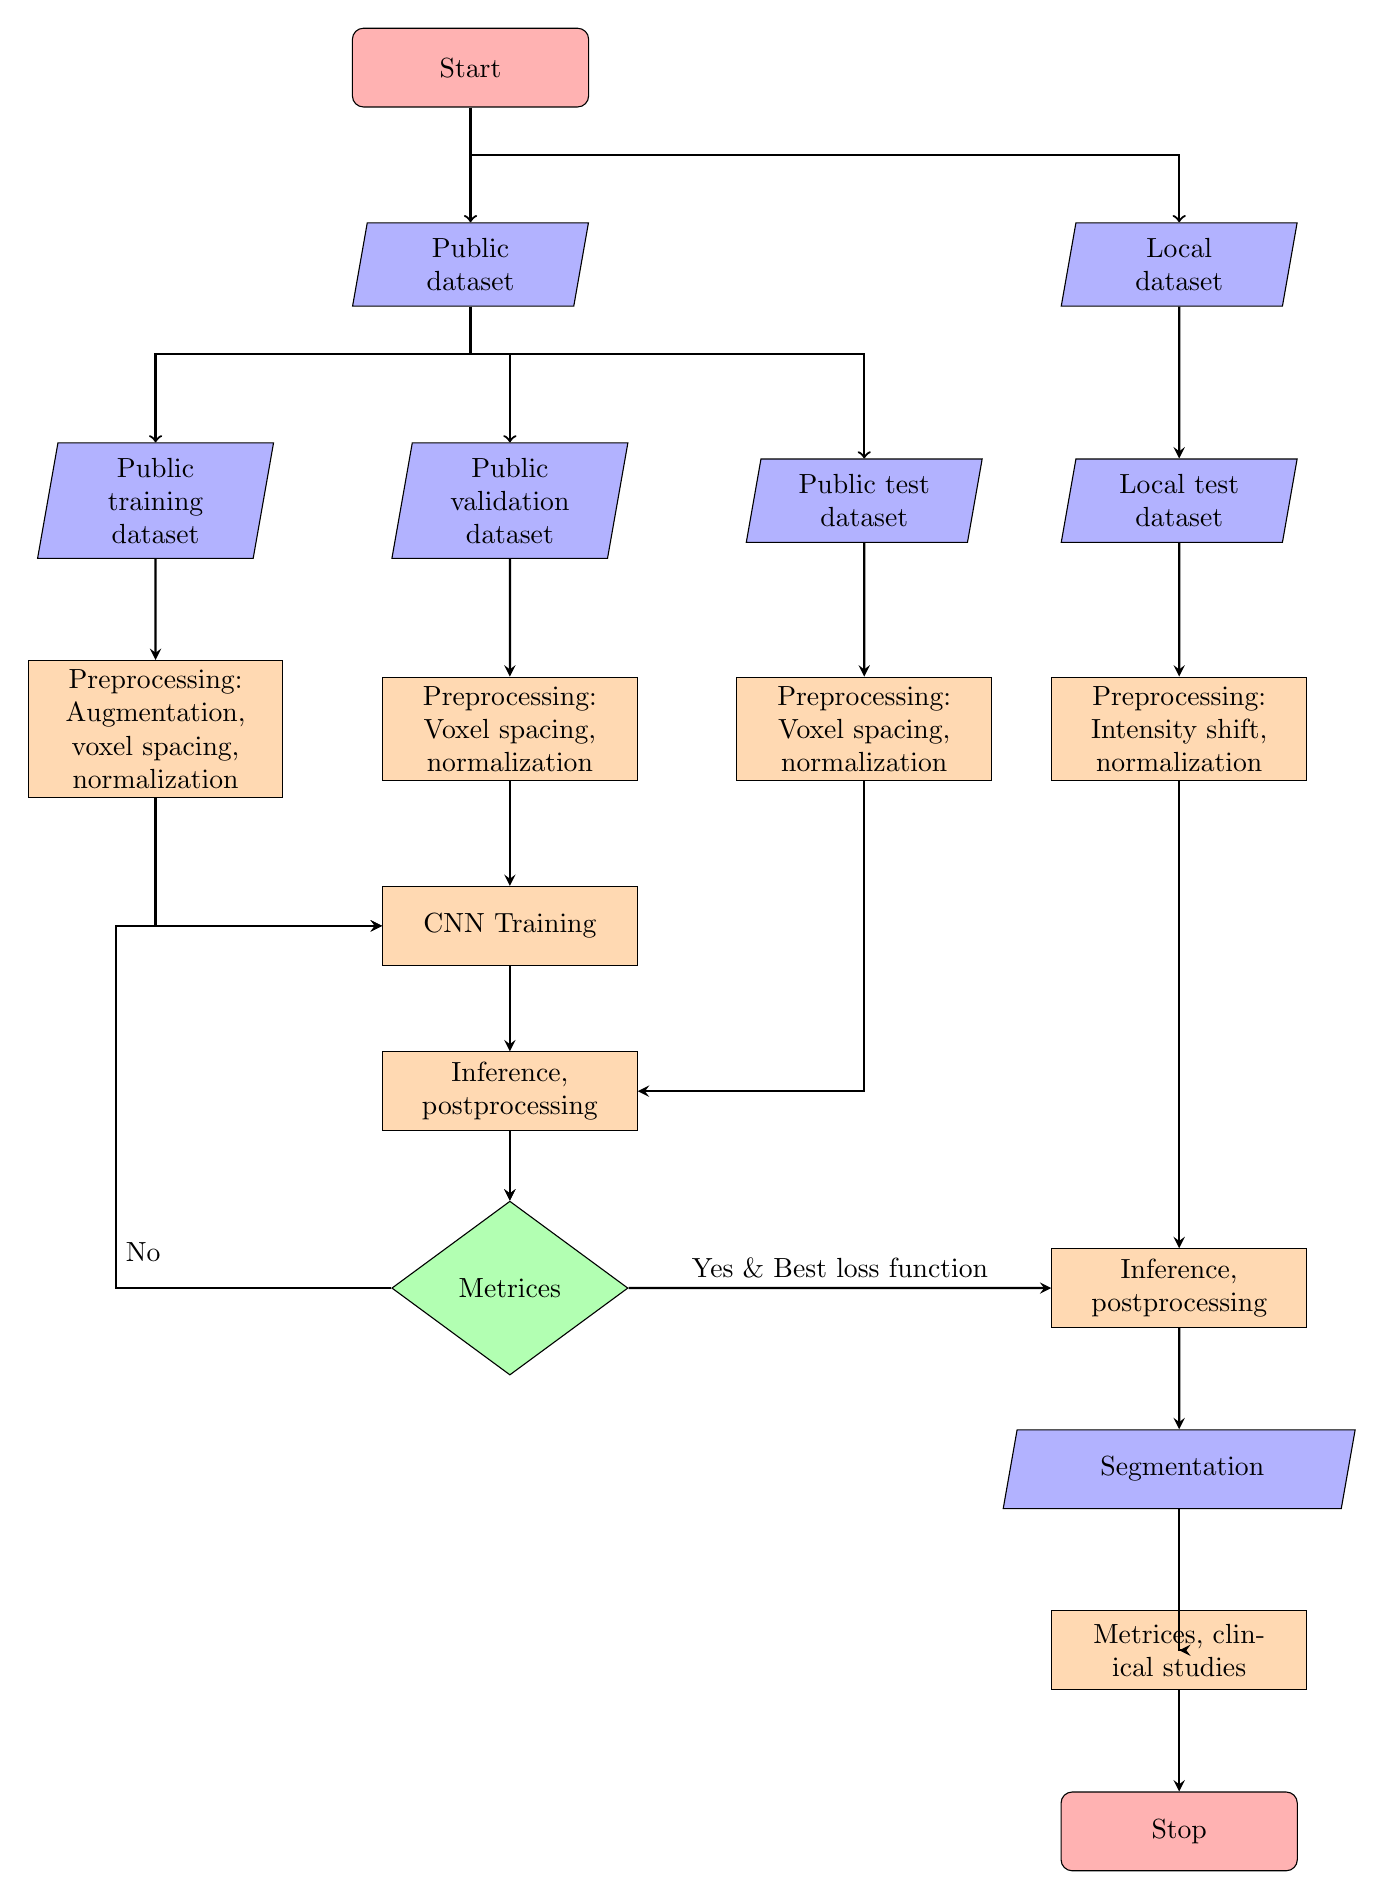
\begin{tikzpicture}[node distance=2cm]
\node (start) [startstop ] {Start};
\node (pdata) [io, below of=start, yshift=-0.5cm] {Public dataset};
\node (prdata) [io,  right of=pdata, xshift=7cm] {Local dataset};

\node (ptrain) [io, below of=pdata, xshift=-4cm, yshift=-1cm] {Public training dataset};
\node (pv) [io,  right of=ptrain, xshift=2.5cm] {Public validation dataset};
\node (ptest) [io,  right of=pv, xshift=2.5cm] {Public test dataset};
\node (test) [io,  below of=prdata, yshift=-1cm] {Local test dataset};

\node (pretr) [process, below of=ptrain, yshift=-0.9cm] {Preprocessing: Augmentation, voxel spacing, normalization};
\node (prepv) [process, right of=pretr, xshift=2.5cm] {Preprocessing: Voxel spacing, normalization};
\node (prept) [process, right of=prepv, xshift=2.5cm] {Preprocessing: Voxel spacing, normalization};
\node (prel) [process, below of=test, yshift=-0.9cm] {Preprocessing: Intensity shift, normalization};

 \node (AItr) [process, below of=prepv,   yshift=-0.5cm] {CNN Training};
 
  \node (Infer) [process, below of=AItr, yshift=-0.1cm] {Inference, postprocessing};
  
 \node (eval) [decision, below of=Infer, yshift=-0.5cm] {Metrices};
 
 \node (inferT) [process,  below of=prel, yshift=-5.1cm] {Inference, postprocessing};
\node (out) [io,  below of=inferT, yshift=-0.3cm] {Segmentation};
\node (analys) [process,  below of=out, yshift=-0.3cm] {Metrices, clinical studies};
\node (stop) [startstop,  below of=analys, yshift=-0.3cm] {Stop};
\draw[thick,->] (start.south) - ++ (0,-0.6cm) -| node[left]  {} (pdata);
\draw[thick,->] (start.south) - ++ (0,-0.6cm) -| node[right] {} (prdata);	
\draw [arrow] (prdata) -- (test);
\draw[thick,->] (pdata.south) - ++ (0,-0.6cm) -| node[left]  {} (ptrain);
\draw[thick,->] (pdata.south) - ++ (0,-0.6cm) -| node[right] {} (ptest);
\draw[thick,->] (pdata.south) - ++ (0,-0.6cm) -| node[right] {} (pv);
\draw [arrow] (test) -- (prel);

\draw [arrow] (ptrain) -- (pretr);
\draw [arrow] (pv) -- (prepv);
\draw [arrow] (ptest) -- (prept);
 \draw [arrow] (pretr) |- (AItr);
  \draw [arrow] (prepv) -- (AItr);
 \draw [arrow] (prept) |- (Infer);
 \draw [arrow] (AItr) -- (Infer);
 \draw [arrow] (Infer) -- (eval);
 \draw [arrow] (Infer) -- (eval);
 
 \draw [arrow] (eval) --node[anchor=south] {Yes \& Best loss function }(inferT);
 \draw [arrow] (eval.west) -- ++(-3.5,0) |- node[right, pos=0.05] {No} (AItr.west);
 
\draw [arrow] (prel) -- (inferT);
 \draw [arrow] (inferT) -- (out); 
 \draw [arrow] (out) |- (analys);  
 \draw [arrow] (analys) -- (stop);         
 
	\end{tikzpicture}
	

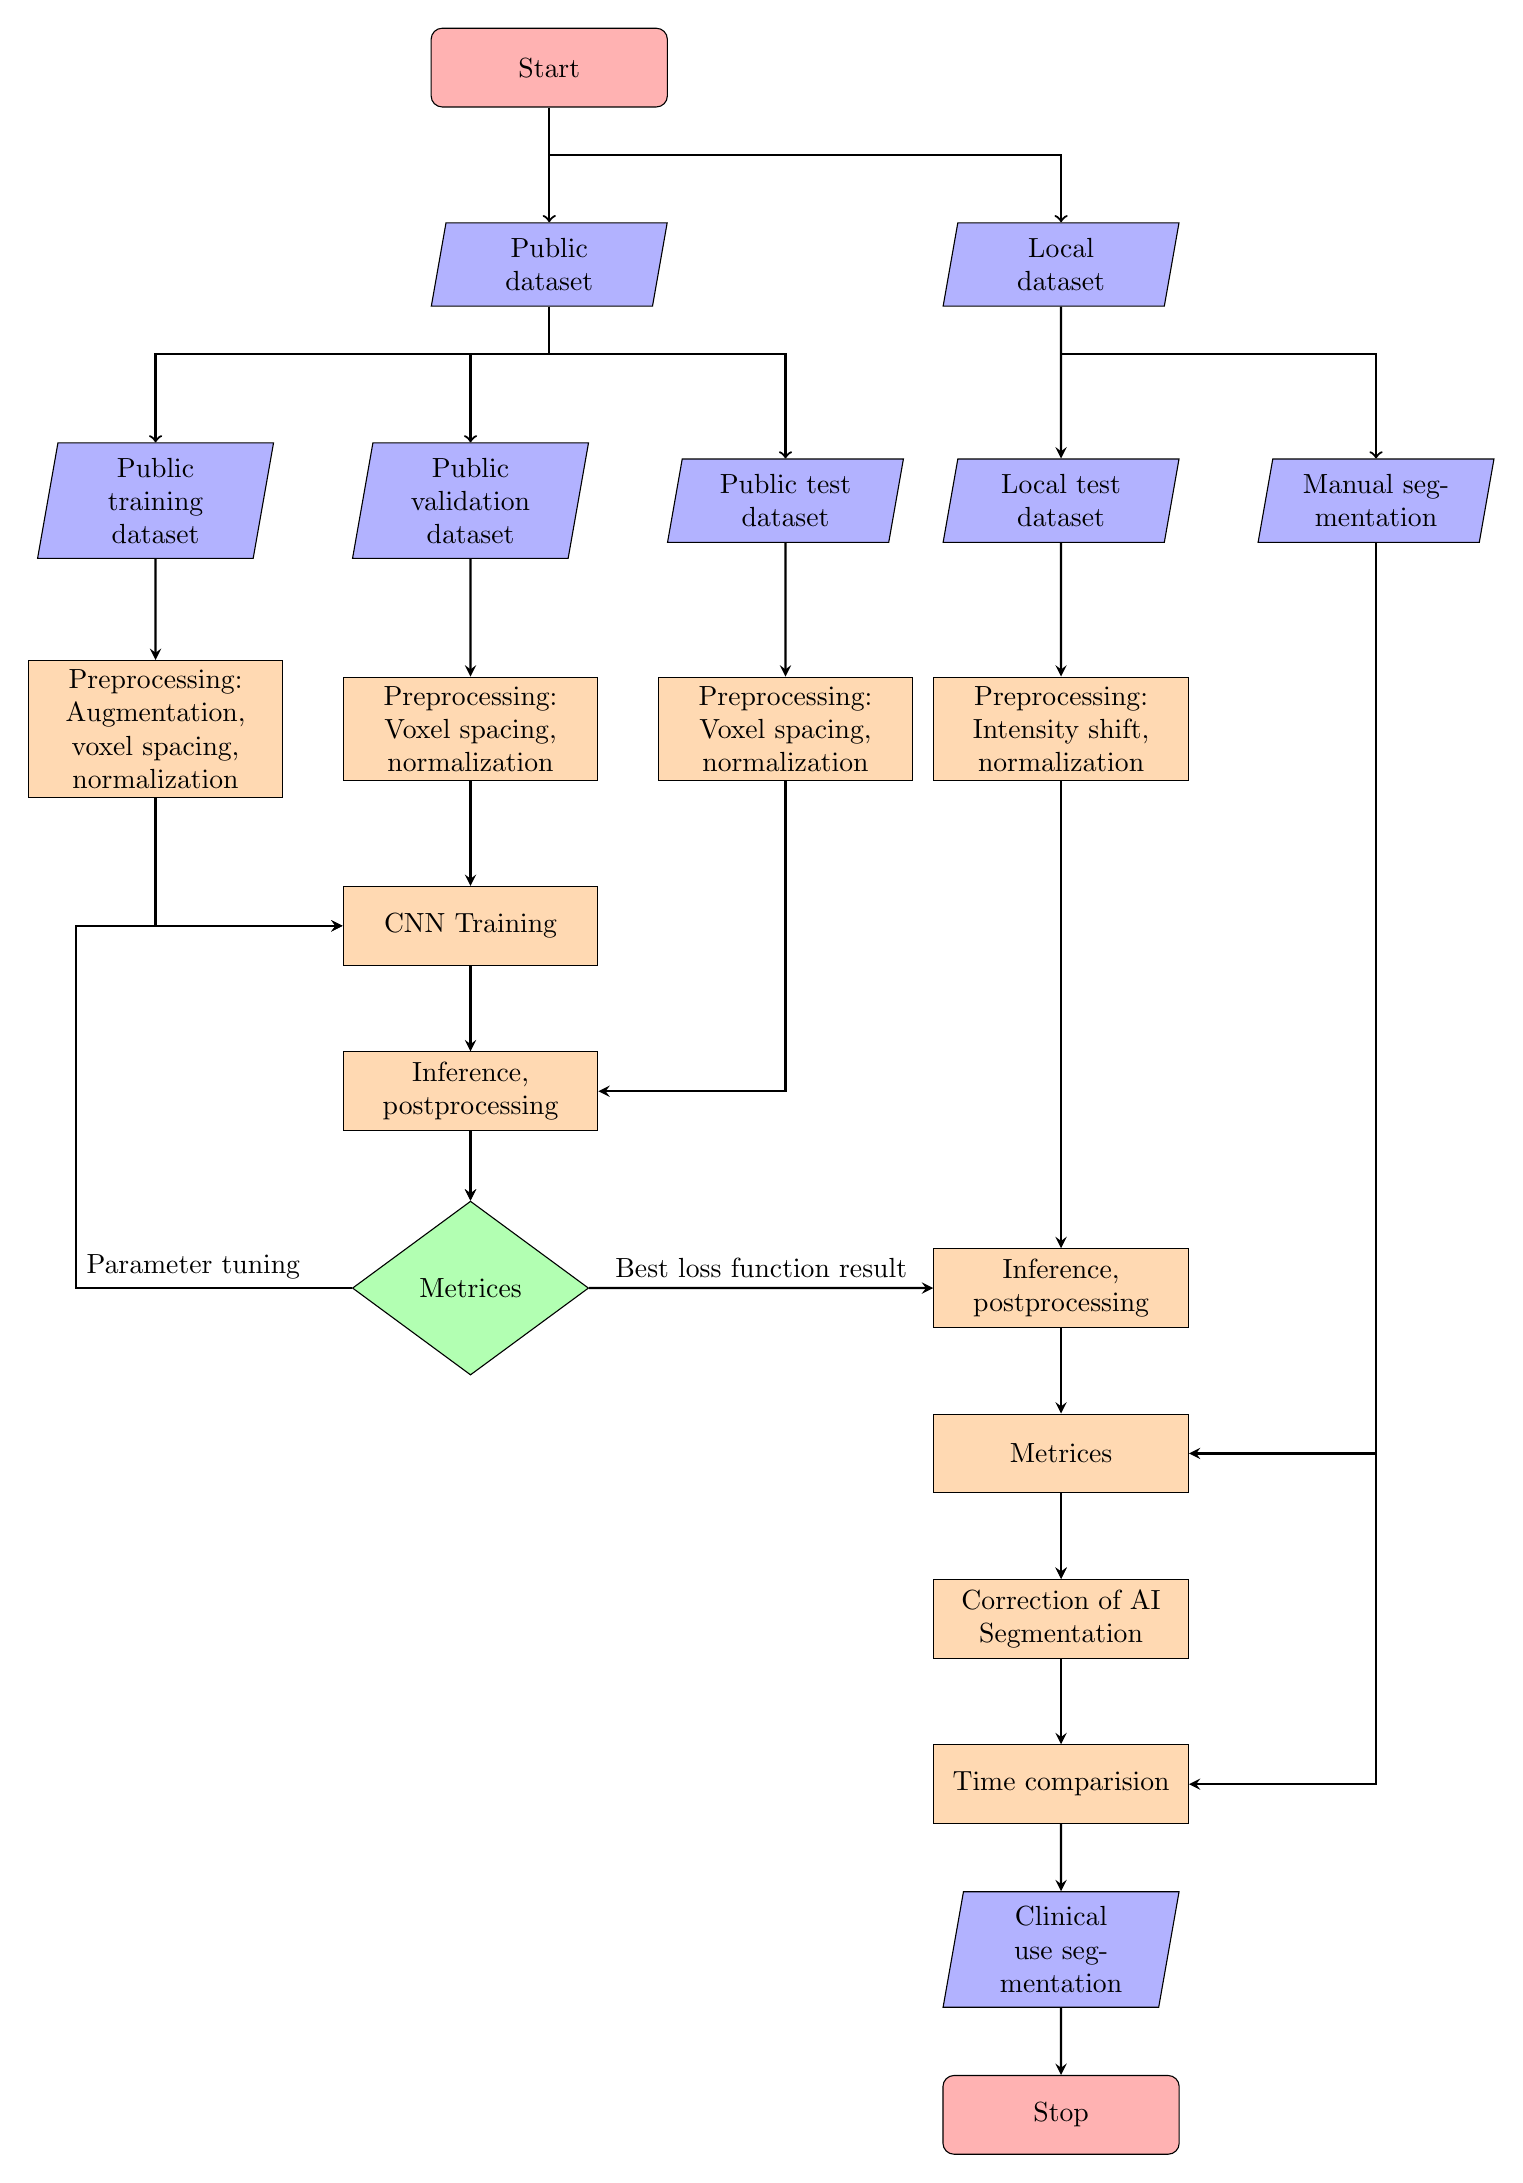
\begin{tikzpicture} [node distance=2cm] 
\node (start) [startstop ] {Start};
\node (pdata) [io, below of=start, yshift=-0.5cm] {Public dataset};
\node (prdata) [io,  right of=pdata, xshift=4.5cm] {Local     dataset};

\node (ptrain) [io, below of=pdata, xshift=-5cm, yshift=-1cm] {Public training dataset};
\node (pv) [io,  right of=ptrain, xshift=2cm] {Public validation dataset};
\node (ptest) [io,  right of=pv, xshift=2cm] {Public test dataset};
\node (test) [io,  below of=prdata, yshift=-1cm] {Local test dataset};
\node (rseg) [io,  right of=test, xshift=2cm] {Manual segmentation};


\node (pretr) [process, below of=ptrain, yshift=-0.9cm] {Preprocessing: Augmentation, voxel spacing, normalization};
\node (prepv) [process, right of=pretr, xshift=2cm] {Preprocessing: Voxel spacing, normalization};
\node (prept) [process, right of=prepv, xshift=2cm] {Preprocessing: Voxel spacing, normalization};
\node (prel) [process, below of=test, yshift=-0.9cm] {Preprocessing: Intensity shift, normalization};

\node (AItr) [process, below of=prepv,   yshift=-0.5cm] {CNN Training};

\node (Infer) [process, below of=AItr, yshift=-0.1cm] {Inference, postprocessing};

\node (eval) [decision, below of=Infer, yshift=-0.5cm] {Metrices};

\node (inferT) [process,  below of=prel, yshift=-5.1cm] {Inference, postprocessing};
\node (out) [process,  below of=inferT, yshift=-0.1cm] {Metrices};
\node (analys) [process,  below of=out, yshift=-0.1cm] {Correction of AI Segmentation};
\node (time) [process,  below of=analys, yshift=-0.1cm] {Time comparision};
\node (use) [io,  below of=time, yshift=-0.1cm] {Clinical use segmentation};

\node (stop) [startstop,  below of=use, yshift=-0.1cm] {Stop};
\draw[thick,->] (start.south) - ++ (0,-0.6cm) -| node[left]  {} (pdata);
\draw[thick,->] (start.south) - ++ (0,-0.6cm) -| node[right] {} (prdata);

\draw[thick,->] (prdata.south) - ++ (0,-0.6cm) -| node[right] {} (rseg);
\draw [arrow] (prdata) -- (test);
\draw[thick,->] (pdata.south) - ++ (0,-0.6cm) -| node[left]  {} (ptrain);
\draw[thick,->] (pdata.south) - ++ (0,-0.6cm) -| node[right] {} (ptest);
\draw[thick,->] (pdata.south) - ++ (0,-0.6cm) -| node[right] {} (pv);
\draw [arrow] (test) -- (prel);

\draw [arrow] (ptrain) -- (pretr);
\draw [arrow] (pv) -- (prepv);
\draw [arrow] (ptest) -- (prept);
\draw [arrow] (pretr) |- (AItr);
\draw [arrow] (prepv) -- (AItr);
\draw [arrow] (prept) |- (Infer);
\draw [arrow] (AItr) -- (Infer);
\draw [arrow] (Infer) -- (eval);
\draw [arrow] (Infer) -- (eval);

\draw [arrow] (eval) --node[anchor=south] {Best loss function result  }(inferT);
\draw [arrow] (rseg) |- (out);

\draw [arrow] (eval.west) -- ++(-3.5,0) |- node[right, pos=0.03] {Parameter tuning} (AItr.west);

\draw [arrow] (prel) -- (inferT);
\draw [arrow] (inferT) -- (out); 
\draw [arrow] (out) -- (analys);  
\draw [arrow] (out) -- (analys);  
\draw [arrow] (analys) -- (time);  
\draw [arrow] (rseg) |- (time);
\draw [arrow] (time) -- (use);  
\draw [arrow] (use) -- (stop);         
\end{tikzpicture}
\end{document}
%